\documentclass{article}
\usepackage[left=3cm,right=3cm,top=3cm,bottom=3cm]{geometry}
\usepackage[utf8]{inputenc}
\usepackage{amsmath}
\usepackage{graphicx}

\DeclareMathOperator{\sequencer}{\textbf{Sequencer}{<}\textbf{N}{>}}
\DeclareMathOperator{\alternator}{\textbf{Alternator}{<}\textbf{N}{>}}
\DeclareMathOperator{\earep}{\textbf{EAReplicator}{<}\textbf{N}{>}}
\DeclareMathOperator{\eaoseq}{\textbf{EAOSequencer}{<}\textbf{N}{>}}

\title{Benchmarking the C interface of the Reo-Rust compiler}
\author{Max Blankestijn, Loes Dekker \& Rintse van de Vlassakker}
\date{March 2020}

\begin{document}

\maketitle

%TODO? \input ipv \include insert the .tex file op dezelfde page
\section{Introduction}
Many programs are comprised of different parallel processes that need to synchronize, communicate, or pass messages. Such behavior can be expressed as a protocol defining the data flow between different processes. Current implementations of such behavior use near archaic programming paradigms such as mutexes, semaphores, monitors, etc. Such implementations are generally implemented on a low level within the code of the components, making modification or verifying the higher level protocol disproportionately difficult.\\
The Reo Coordination Language \cite{reo} allows the specification of a high level protocol separate from the implementation of different processes. This allows easy modification of protocols and allows them to be ported to different applications by simply exchanging the corresponding processes. \\\\
%
Using the current build of the Reo Compiler \cite{reo:git} we will build several circuits and benchmark them. These will be compared to a similar C\texttt{++} implementation that implements the same circuits.\\
We will provide a specification of the protocols and describe their behavior, which we will follow with a description of our experiments and the used hardware. Lastly our gathered results will be provided and discussed.

\section{Protocols} \label{sec:protocols}
We consider four protocols with different types of behaviour. This section will describe these protocols and provide a specification of their behaviour using both reo circuits \cite{puff} and timed-data-stream seamntics \cite{datastream}.

\subsection{Sequencer}%
\begin{minipage}{.65\textwidth}
  This protocol ensures that N producers fire in a cyclic sequence.\\\\
  %
  It has the following data stream semantics:\\\\
  %
  $
  \vspace{0.2cm}\sequencer (\langle \alpha_0, a_0 \rangle, \langle \alpha_1, a_1 \rangle,\;...\; \langle \alpha_{\textbf{N}-1}, a_{\textbf{N}-1} \rangle) \equiv \\
  \vspace{0.2cm}\hphantom \qquad  \alpha_0(0) < \alpha_1(0) < ... < \alpha_{\textbf{N}-1}(0) < \alpha_0(1) \\
  \hphantom \qquad \sequencer(\langle \alpha_0', a_0' \rangle, \langle \alpha_1', a_1' \rangle,\;...\; \langle \alpha_{N-1}', a_{\textbf{N}-1}' \rangle)
  $
\end{minipage}\hfill
\begin{minipage}{.25\textwidth}
  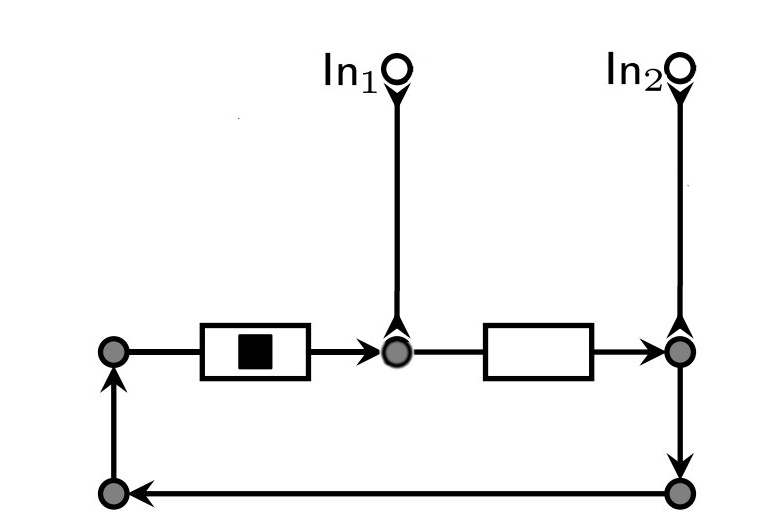
\includegraphics[width=5cm]{img/seq.png}
\end{minipage}

\subsection{Alternator}
\begin{minipage}{.65\textwidth}
  This protocol waits for all N inputs to put and the one output to get, after which the data of the first producer is instantly consumed.
  All the other producers have their output buffered, and consumed one by one in a set order.
  Only after all data has been consumed, may the producers fire again.\\\\
  %
  It has the following data stream semantics:\\\\
  %
  $
  \vspace{0.2cm} \alternator (\langle \alpha_0, a_0 \rangle, \langle \alpha_1, a_1 \rangle,\; ... \; \langle \alpha_{\textbf{N}-1}, a_{\textbf{N}-1} \rangle; \langle \beta, b \rangle) \equiv \\
  \vspace{0.2cm} \hphantom \qquad \alpha_0(0) = \alpha_1(0) = ... = \alpha_{\textbf{N}-1}(0) =\\
  \vspace{0.2cm} \hphantom \qquad \beta(0) < \beta(1) < ... < \beta(\textbf{N}-1) < \alpha_0(1) \\
  \vspace{0.2cm} \hphantom \qquad\forall 0 \leq i < \textbf{N} :\quad b(i) = a_i(0) \\
  \hphantom \qquad \alternator (\langle \alpha_0', a_0' \rangle, \langle \alpha_1', a_1' \rangle,\;...\; \langle \alpha_{N-1}', a_{N-1}' \rangle; \langle \beta(\textbf{N},\;...), b(\textbf{N},\;...) \rangle)
  $

\end{minipage}\hfill
\begin{minipage}{.25\textwidth}
  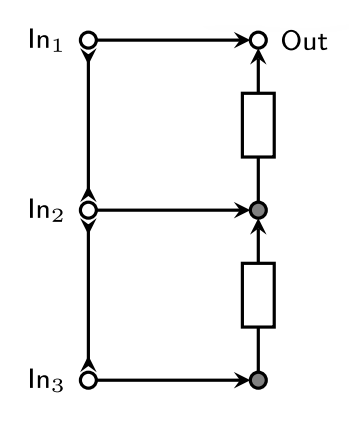
\includegraphics[width=4cm]{img/alt.png}
\end{minipage}

\subsection{Early Async Replicator}
\begin{minipage}{.65\textwidth}
  This protocol has one producer, whose data is buffered when put, and $N$ consumers, which all replicate the producers data.
  All consumers fire simultaneously, but strictly after the producer.\\\\
  %
  It has the following data stream semantics:\\\\
  %
  $
  \vspace{0.2cm}\earep (\langle \alpha, a \rangle ; \langle \beta_0, b_0 \rangle, \langle \beta_1, b_1 \rangle,\; ... \; \langle \beta_{\textbf{N}-1}, b_{\textbf{N}-1} \rangle) \equiv \\
  \vspace{0.2cm} \hphantom \qquad \forall 0 \leq i < \textbf{N} : \quad \alpha(0) < \beta_i(0) < \alpha(1) \land a(0) = b_i(0) \\
  \hphantom \qquad\forall 0 \leq i < \textbf{N}-1 :\quad \beta_i(0) = \beta_{i+1}(0)
  $
\end{minipage}\hfill
\begin{minipage}{.25\textwidth}
  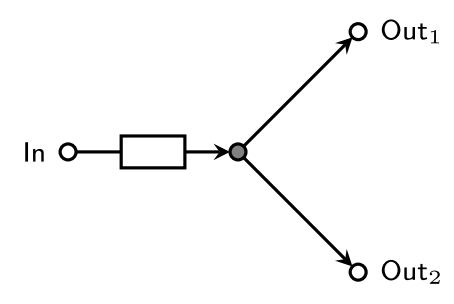
\includegraphics[width=5cm]{img/EARep.png}\\
\end{minipage}

\subsection{Early Async Out Sequencer}
\begin{minipage}{.65\textwidth}
  Given one producer and multiple consumers, this protocol saves a production to a buffer and then directs it to one consumer. The consumers fire in a set order.\\\\
  %
  It has the following data stream semantics:\\\\
  %
  $
  \vspace{0.2cm}\eaoseq (\langle \alpha, a \rangle;\langle \beta_0, b_0 \rangle, \langle \beta_1, b_1 \rangle,\;...\; \langle \beta_{\textbf{N}-1}, b_{\textbf{N}-1} \rangle) \equiv
  \vspace{0.2cm} \hphantom \qquad \alpha(0) < \beta_0(0) < \alpha(1) \land a(0) = b_0(0) \\
  \hphantom \qquad \eaoseq (\langle \alpha', a' \rangle; \langle \beta_1, b_1 \rangle,\langle \beta_2, b_2 \rangle,\;...\; \langle \beta_{\textbf{N}-1}, b_{\textbf{N}-1} \rangle, \langle \beta_0', b_0' \rangle)
  $
\end{minipage}\hspace{0.05cm}
\begin{minipage}{.25\textwidth}
  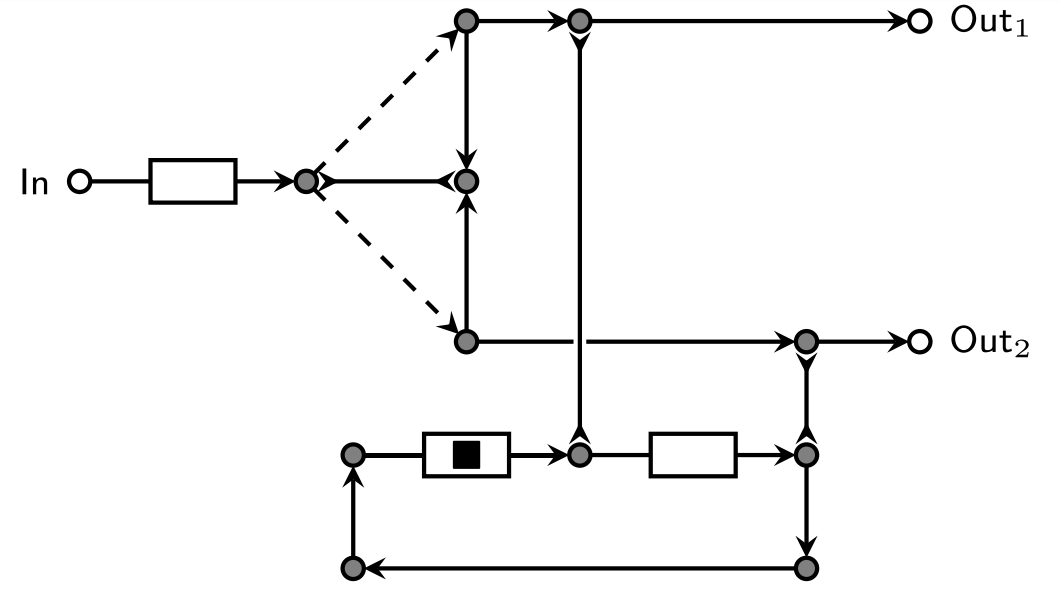
\includegraphics[width=7cm]{img/eaoseq.png}\\
\end{minipage}

\section{Materials}
\subsection{Treo Compiler}
Reo protocols can be specified using its automata type circuits but in order convert a protocol into functioning code a textual representation is required. The Treo \cite{treo} compiler \cite{reo:git} converts a textual reo protocol into a target language and connects the input and output ports to code provided by the user.

\subsection{Reo\_rs Compiler}
The Reo Rs \cite{reors:git} allows textual reo protocols to determine data flow in Rust and C programs. It outputs a Rust source file or C library based on the supplied treo protocol.

\subsection{Hardware}

section{Implementation}

We designed our own Implementations of these protocols as classes in C++. The classes have a put() and get() function that behave just like a put and get to a port in a Reo protocol. We made sure that a thread blocks and conintues in the put() and get() functions just like a Reo protocol would block when getting and putting. To actually implement the protocol's logic, we used the POSIX threads library. This is a low level threading library that would most likely be used in any application where speed is of importance.

\section{Experiments}
The protocols from section \ref{sec:protocols} are implemented using Treo, section \ref{sec:treo}, for the exact implementation see \verb|treo/treo| in \cite{us:git}. The Rust source and C library are given a series of different sizes, which will scale the amount consumers or producers of a protocol. The Sequencer and Alternator will scale the amount of producers, as there is only a single output port and variable inputs. The Early Async Replicator and Early Async Out Sequencer only scale their consumers, since here the input is constant.\\
The same will be done for our hand crafted C\texttt{++} code.\\\\
%
Due to issues with the compiler not all protocols and input sizes were able to be compiled and run. This report will contain all successful runs and omit the rest. The originally planned input parameters were a input/output size of 4, 16, 64, 256, 512, and 1024.

\section{Conclusion and Further Research}


\newpage
\bibliographystyle{alpha}
\bibliography{bibliography}

\end{document}
